\documentclass{standalone}
\usepackage{tikz}
\usepackage{graphicx}
\usepackage{pgffor}
\definecolor{joired}{RGB}{218,11,49}
\definecolor{joigreen}{RGB}{18,136,104}
\definecolor{joiyellow}{RGB}{250,210,49}
\definecolor{joiblue}{RGB}{15,105,180}
\definecolor{joiblack}{RGB}{0,0,1}

\begin{document}
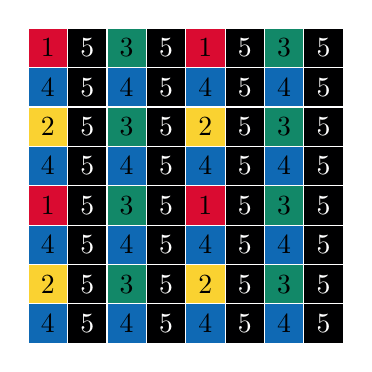
\begin{tikzpicture}

\foreach \y in {0, 1, 2, ..., 7}{
	\foreach \x in {1, 3, 5, 7}{
		\fill[joiblack] (0.5*\x, 0.5*\y) rectangle +(0.5, 0.5);
		\node at (0.25+0.5*\x, 0.25+0.5*\y) {\color{white} 5};
	}
}

\foreach \y in {0, 2, 4, 6}{
	\foreach \x in {0, 2, 4, 6}{
		\fill[joiblue] (0.5*\x, 0.5*\y) rectangle +(0.5, 0.5);
		\node at (0.25+0.5*\x, 0.25+0.5*\y) {4};
	}
}

\foreach \y in {1, 3, 5, 7}{
	\foreach \x in {2, 6}{
		\fill[joigreen] (0.5*\x, 0.5*\y) rectangle +(0.5, 0.5);
		\node at (0.25+0.5*\x, 0.25+0.5*\y) {3};
	}
}

\foreach \y in {1, 5}{
	\foreach \x in {0, 4}{
		\fill[joiyellow] (0.5*\x, 0.5*\y) rectangle +(0.5, 0.5);
		\node at (0.25+0.5*\x, 0.25+0.5*\y) {2};
	}
}


\foreach \y in {3, 7}{
	\foreach \x in {0, 4}{
		\fill[joired] (0.5*\x, 0.5*\y) rectangle +(0.5, 0.5);
		\node at (0.25+0.5*\x, 0.25+0.5*\y) {1};
	}
}

\draw[step=0.5, white] (0,0) grid (4,4);
\end{tikzpicture}
\end{document}